\section{Finite Differencing}\label{chap:finitediff}
%
\paragraph{Hemispheric symmetry}
%
As mentioned in section \ref{cap:electro_equ} we assume that the conductivity 
along the magnetic field line is
very large, thus conjugate foot points are equipotential. To get a symmetric
potential pattern we add the conductances and wind driven current densities of
the two hemispheres together and solve for only one.
The symmetry of the potential pattern is only valid at low-- and
mid--latitudes with closed field lines. At high latitudes 
the electric potential is specially treated as
discussed in section \ref{cap:high_lat}. \\

%
The added together values from the northern and southern hemisphere 
 are denoted by $(\cdot)^T$ (see equation 
(\ref{eq:nh_1})--(\ref{eq:nh_6})). In the source code in
\texttt{subroutine dynamo} the following values are calculated
%
\begin{align}
   \Sigma_{\phi \phi}^T(0)      &= \Sigma_{\phi \phi}^{NH}(0) + \Sigma_{\phi \phi}^{SH}(0)\\
   \Sigma_{\lambda \lambda}^T(0)&=\Sigma_{\lambda \lambda}^{NH}(0)+ \Sigma_{\lambda \lambda}^{SH}(0) \\
  -\Sigma_{C}^T(0)&= -(\Sigma_{C}^{NH}(0)-\Sigma_{C}^{SH}(0))\\
   \Sigma_{H}^T(0)&=   \Sigma_{H}^{NH}(0)-\Sigma_{H}^{SH}(0)\\
   K_{m \phi}^{DT}(0)    &= K_{m \phi}^{D,NH}(0)+ K_{m \phi}^{D,SH}(0)\\
   K_{m \lambda}^{DT}(0) &= K_{m \lambda}^{D,NH}(0)-K_{m \lambda}^{D,SH}(0)
\end{align}
%
Note that in the source code $-\Sigma_{C}^T(0)$ is put into ZIGMC, and that
$-K_{m \lambda}^{D,SH}(0)$ was saved in RIM(2). The hemispherically added values are 
saved in the latitude indices of
the northern hemisphere from $(nmlat+1)/2$, which is the index for the equator, to
the pole at $nmlat$. The number of magnetic latitudes 
is $nmlat$.
%
\paragraph{Differencing of the right hand side}\label{page:finite_rhs}
%
In \texttt{subroutine rhspde} the right hand side is differentiated. 
%
\begin{equation}
   rhs = \frac{R_0}{cos \lambda_0} \bigl[ \frac{\partial K_{m \phi}^{DT}(0)}{\partial \phi_0} +  
   \frac{\partial K_{m \lambda }^{DT}(0) cos \lambda_0}{\partial | \lambda_0 |}
   \bigr] \label{eq:diff_rhs}
\end{equation}
%
A central differencing scheme is used which leads to the derivative at the location 
$\phi(i)$, $\lambda_0(j)$
%
\begin{equation}
\begin{split}
  rhs(i,j) = & \frac{R_0}{ 2 \Delta \phi cos \lambda_0(j)} \bigl[ K_{m \phi}^{DT}(0)(i+1,j) - 
      K_{m \phi}^{DT}(0)(i-1,j)\bigr] + \\
   & \frac{R_0}{ 2 \Delta \lambda_0 cos \lambda_0(j)} \bigl[ K_{m \lambda }^{DT}(0)(i,j+1) 
    cos \lambda_0(j+1)- \\
    &  K_{m \lambda }^{DT}(0)(i,j-1)cos \lambda_0(j-1) \bigr] 
\end{split}
\end{equation}
%
with i, j the longitudinal and latitudinal index and the adjacent grid points $i\pm 1$,$j \pm1$.
The polar derivative is approximated by
%
\begin{equation}
   rhs (i,j_{pole}) = - \frac{2 R_0}{cos \lambda_0(j-1) mlon} \bigl[ \sum_{i=1}^{mlon} 
       K_{m \lambda }^{DT}(0)(i,j_{pole} - 1)  \bigr]
\end{equation}
%
At the magnetic equator the northward current $K_{m \lambda} $ has to
vanish see equation (\ref{eq:kmlamequator}) or  in \cite{rich95} eq. (5.30)
or (5.31). Therefore the right hand side derivatives are discretized by
%
\begin{equation}
  \begin{split}
  rhs(i,j_{eq}) =&  \frac{R_0}{  \Delta \phi cos \lambda_0(j_{eq})} \bigl[ K_{m \phi}^{D, mod T}(0)(i+\frac{1}{2},j_{eq}) - 
      K_{m \phi}^{D, mod T}(0)(i-\frac{1}{2},j_{eq})\bigr] + \\
     &\frac{2 R_0}{ \Delta \lambda_0 } \bigl[ K_{m \lambda }^{DT}(0)(i,j_{eq}+\frac{1}{2}) 
    cos \lambda_0(j_{eq}+\frac{1}{2}) \bigr] \label{eq:rhs_eq1}
  \end{split}
\end{equation}
%
with $ K_{m \phi}^{D, mod}$ the modified height integrated eastward
current density due to neutral winds $K_{m \phi}^{D}$, see equation 
(\ref{eq:kqphi_mod}). It is referred to section \ref{finite_equator} 
eq. (\ref{eq:finite_eqbnd1})--(\ref{eq:finite_eqbnd3}) for explanation 
of the discrete boundary condition at the magnetic equator. 
At the geomagnetic equator $cos \lambda_0(j_{eq})=1$ and equation (\ref{eq:rhs_eq1}) 
can be written as
%
\begin{equation}
  \begin{split}
  rhs(i,j_{eq}) =& \frac{R_0}{ 2 \Delta \phi_0} \bigl[ K_{m \phi}^{D, mod T}(0)(i+1,j_{eq}) - 
      K_{m \phi}^{D, mod T}(0)(i-1,j_{eq})\bigr] + \\
     &\frac{R_0}{ \Delta \lambda_0 } \bigl[ K_{m \lambda }^{DT}(0)(i,j_{eq}+1) 
    cos \lambda_0(j_{eq}+1) + K_{m \lambda }^{DT}(0)(i,j_{eq} )\bigr]
  \end{split}
\end{equation}
%
The whole right hand side is multiplied by $R_0$ in [m] to get eq. (\ref{eq:diff_rhs}). 
%
\paragraph{Differencing of the left hand side}\label{page:diff_lhs}
%
In this paragraph the finite differencing of the left hand side of the electrodynamo
equation is
discussed. In the source code the calling tree for the differencing is the
following:
%
\begin{verbatim}
subroutine dynamo
...
if (isolve == 2) then
   call stencmd
        call htrpex
        call cnmmod
        call cnm
else
   call stencil
        call htrpex
        call cnm
endif
...
\end{verbatim}
%
The flag  \flags{isolve}=2 means that at the finest grid level an additional coefficient 
matrix is set up  without upwinding for terms violating
the diagonal dominance
(see paragraph further down in this section). The multigrid solver 
which is discussed in section \ref{cap:solve} uses the coefficient 
matrix without upwinding to calculate the residual on the finest
grid level. At all other grid levels the coefficient matrix 
with upwinding is used to solve for the 
residual. If  \flags{isolve}$ \neq 2$ the
upwinding method is applied at all grid levels to solve for the
electric potential. For more information
about the different option with the multigrid solver we refer to 
section \ref{cap:solve}. \\
 
%
In \texttt{subroutine dynamo} the conductances are prepared for the
finite differencing. The conductance coefficients represent 
% 
\begin{align}
A&= \frac{\Sigma_{\phi \phi}^T(0)}{cos\lambda_0  \Delta \phi^2 }	   \rightarrow  zigm11\label{eq:sig_dif1}\\
B&= \frac{\Sigma_{\lambda \lambda}^T(0) cos \lambda_0}{\Delta \lambda_0^2} \rightarrow  zigm22\label{eq:sig_dif2} \\
C&= \frac{\Sigma_{\phi \lambda}^T(0)}{4\Delta \lambda_0 \Delta \phi }    \rightarrow  zigmc \label{eq:sig_dif3} \\
D&= \frac{\Sigma_{\phi \lambda}^T(0)}{4 \Delta \lambda_0 \Delta \phi}    \rightarrow  zigm2 \label{eq:sig_dif4} 
\end{align}
%
with \src{zigm11}, \src{zigm22}, \src{zigmc}, \src{zigm2} the variable names in
the source code.
Note that the factor of four is introduced due to the 
central differencing. Both hemisphere are already added 
together and the coefficients are stored in the index range
of the "northern hemisphere" ((nmlat+1)/2 to nmlat).
In the "southern hemisphere" index range (1 to (nmlat+1)/2), the same values are stored as in the
northern range ((nmlat+1)/2 to nmlat) except of the two mixed terms which change
sign.
% 
\begin{align}
 zigmc(SH)  \rightarrow -\frac{\Sigma_{\phi \lambda}^T(0)}{4\Delta \lambda_0 \Delta \phi } \\
 zigm2(SH)  \rightarrow -\frac{\Sigma_{\phi \lambda}^T(0)}{4 \Delta \lambda_0 \Delta \phi} 
\end{align}
%
The polar value of $\frac{\Sigma_{\phi \phi}^T(0)}{cos\lambda_0  \Delta \phi^2 }$
is set to zero to avoid floating point exception. The polar value is
not used in the electrodynamo equation since the potential at the pole is
prescribed. \\
%
The \texttt{subroutine stencmd} or \texttt{subroutine stencil} is called
for each conductance term eq. (\ref{eq:sig_dif1})--(\ref{eq:sig_dif4}) 
and the finite difference stencil is updated for the contributions 
of the corresponding conductance term. First the conductance
is copied into a working
array in \texttt{subroutine htrpex} and the longitudinal wrap around points, 
necessary for
the longitudinal derivatives, are set. Note that there are 5 different grid
levels and therefore there are 16 additional points on either side of the
working array. The working array stores the values from the equator (index 1) to the pole
(index (nmlat+1)/2). \\
%
The contributions to the stencil from the different conductances are
determined in \texttt{subroutine cnmmod} and/or \texttt{subroutine cnm}.
\texttt{Subroutine cnmmod} is called if the flag \flags{isolve}=2 
is set, and then only for the finest grid level
This subroutine sets
up the coefficient stencil without upwinding method. At all the other grid
levels upwinding may be used if necessary. For 
\flags{isolve} $\neq 2$ all the stencils are determined with upwinding methods
if necessary, which is done in  \texttt{subroutine cnm}.
Please read section \ref{cap:solve} for more information about the different
solver types (flag \flags{isolve}). \\

%
From equation (\ref{eq:edyn3}) and the values in table \ref{tab:transf_quantities}
we get the following left hand side of the electrodynamo equation.
%
\begin{equation}
\begin{split}
 cos \lambda_0 \; lhs=  & \frac{\partial}{\partial \phi_0} 
    \bigl( \frac{\Sigma_{\phi \phi}^T(0)}{cos
   \lambda_0} \frac{\partial \Phi}{\partial \phi_0} + 
   \Sigma_{\phi \lambda}^T(0) \frac{\partial \Phi}{\partial \lambda_0} \bigr) + \\
    & \frac{\partial}
   {\partial  \lambda_0 } \bigl( \Sigma_{\lambda \phi}^T(0)
    \frac{\partial \Phi}{\partial \phi_0} + 
   \Sigma_{\lambda \lambda}^T(0) cos \lambda_0 
   \frac{\partial \Phi}{\partial \lambda_0} \bigr)
    \label{eq:edyn4}
\end{split}
\end{equation}
%
Note that the right hand side $rhs$ in equation (\ref{eq:diff_rhs}) is already divided
by $cos \lambda_0$ therefore we have to include the $cos \lambda_0$ on the left
hand side of eq. (\ref{eq:edyn4}). Replacing 
the two terms in the brackets in eq.  (\ref{eq:edyn4}) by
%
\begin{align}
 T_{\phi}=&  \frac{\Sigma_{\phi \phi}^T(0)}{cos
   \lambda_0} \frac{\partial \Phi}{\partial \phi_0} + 
   \Sigma_{\phi \lambda}^T(0) \frac{\partial \Phi}{\partial \lambda_0} \label{eq:tphi}\\
 T_{\lambda}=& \Sigma_{\lambda \phi}^T(0)
    \frac{\partial \Phi}{\partial \phi_0} + 
   \Sigma_{\lambda \lambda}^T(0) cos \lambda_0 
   \frac{\partial \Phi}{\partial \lambda_0} \label{eq:tlambda}
\end{align}
%
 leads to
%
\begin{equation}
 cos \lambda_0 \; lhs=  \frac{\partial}{\partial \phi_0} T_{\phi}  +
   \frac{\partial}{\partial  \lambda_0 } T_{\lambda}  \label{eq:edyn5}
\end{equation}
%
For clarity we will omit the dependence on $\lambda_0$ shown by
$(\cdot)(0)$ in the following e.g. we write $\Sigma_{\phi \lambda}^T$ instead off
$\Sigma_{\phi \lambda}^T(0)$. 
Using central differencing for the finite differences gives
%
\begin{equation}
 cos \lambda_0 \; lhs=  \frac{T_{\phi}(i+\frac{1}{2},j)-T_{\phi}(i-\frac{1}{2},j)}
 {\Delta \phi_0}   +
   \frac{ T_{\lambda}(i,j+\frac{1}{2})- T_{\lambda}(i,j-\frac{1}{2})}
   {\Delta  \lambda_0 } \label{eq:edyn6}
\end{equation}
%
with
%
\begin{align}
\begin{split}
 T_{\phi}(i+\frac{1}{2},j)=&  \frac{\Sigma_{\phi \phi}^T(i+\frac{1}{2},j)}{cos
   \lambda_0(j)} \frac{ \Phi(i+1,j)- \Phi(i,j)}{\Delta \phi_0} + \\
   &\Sigma_{\phi \lambda}^T(i+\frac{1}{2},j) 
   \frac{ \Phi(i+\frac{1}{2},j+\frac{1}{2})-\Phi(i+\frac{1}{2},j-\frac{1}{2})}{\Delta \lambda_0}  \\
 T_{\phi}(i-\frac{1}{2},j)=&  \frac{\Sigma_{\phi \phi}^T(i-\frac{1}{2},j)}{cos
   \lambda_0(j)} \frac{ \Phi(i,j)- \Phi(i-1,j)}{\Delta \phi_0} + \\
   &\Sigma_{\phi \lambda}^T(i-\frac{1}{2},j) 
   \frac{ \Phi(i-\frac{1}{2},j+\frac{1}{2})-\Phi(i-\frac{1}{2},j-\frac{1}{2})}{\Delta \lambda_0}  \\
 T_{\lambda}(i,j+\frac{1}{2})=& \Sigma_{\lambda \phi}^T(i,j+\frac{1}{2})
    \frac{ \Phi(i+\frac{1}{2},j+\frac{1}{2})- \Phi(i-\frac{1}{2},j+\frac{1}{2})}{\Delta \phi_0} +\\
   &\Sigma_{\lambda \lambda}^T(i,j+\frac{1}{2}) cos \lambda_0(j+\frac{1}{2}) 
   \frac{ \Phi(i,j+1)-\Phi(i,j)}{\Delta \lambda_0}  \\
 T_{\lambda}(i,j-\frac{1}{2})=& \Sigma_{\lambda \phi}^T(i,j-\frac{1}{2})
    \frac{ \Phi(i+\frac{1}{2},j-\frac{1}{2})- \Phi(i-\frac{1}{2},j-\frac{1}{2})}{\Delta \phi_0} +\\ 
   &\Sigma_{\lambda \lambda}^T(i,j-\frac{1}{2}) cos \lambda_0(j-\frac{1}{2}) 
   \frac{ \Phi(i,j)-\Phi(i,j-1)}{\Delta \lambda_0} 
\end{split}
\end{align}
%
The numbering of the nine point stencil can be seen in figure \ref{fig:stencil}
with the index i denoting the longitude and the index j for the latitude.
%
\begin{figure}
  \centering
  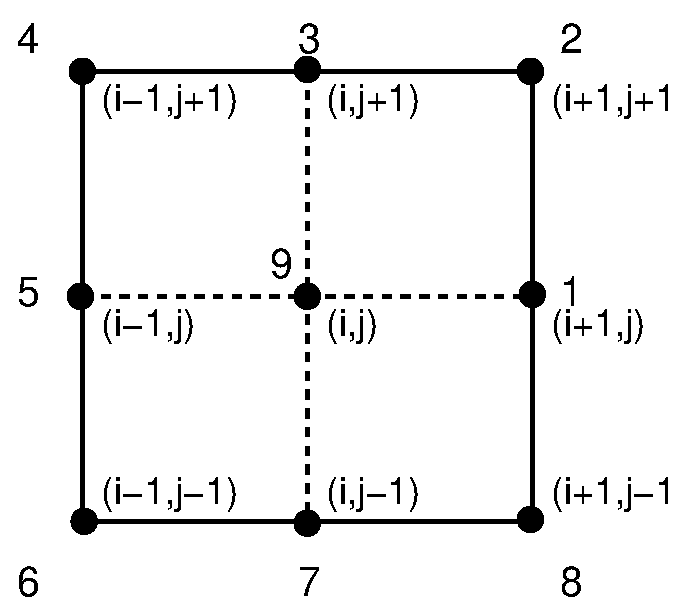
\includegraphics[scale=0.5]{./tex_plot/stencil.eps}
  \caption{Geometry for the 9 point stencil}
   \label{fig:stencil}
\end{figure}
%
The values at half grid points e.g. $(i+\frac{1}{2},j)$ are determined
by averaging the values of the adjacent grid points, e.g.
%
\begin{equation}
 \Sigma_{\phi \phi}^T(i+\frac{1}{2},j) = \frac{1}{2}
   \bigl[ \Sigma_{\phi \phi}^T(i+1,j) +  \Sigma_{\phi \phi}^T(i,j) \bigr]
\end{equation}
%
Accordingly, the values at $(i-\frac{1}{2},j)$, $(i,j+\frac{1}{2})$ and
$(i,j-\frac{1}{2})$ can be calculated. The difference at half points
in latitude and longitude e.g.  $(i+\frac{1}{2},j+\frac{1}{2})$
is also resolved by averaging the values of the adjacent grid 
points which leads to e.g.
%
\begin{equation}
\begin{split}
 &\Phi(i+\frac{1}{2},j+\frac{1}{2}) - \Phi(i+\frac{1}{2},j-\frac{1}{2}) =  \\
 &  \frac{1}{4}
   \bigl[ \Phi(i+1,j+1) -\Phi(i+1,j-1) + \Phi(i,j+1)- \Phi(i,j-1) \bigr]
\end{split}
\end{equation}
%
Accordingly, $\Phi(i-\frac{1}{2},j+\frac{1}{2}) - \Phi(i-\frac{1}{2},j-\frac{1}{2})$,
$\Phi(i+\frac{1}{2},j+\frac{1}{2}) - \Phi(i-\frac{1}{2},j+\frac{1}{2})$ and
$\Phi(i+\frac{1}{2},j-\frac{1}{2}) - \Phi(i-\frac{1}{2},j-\frac{1}{2})$ are discretized.
The resulting contributions from the conductance terms to the nine 
point stencil in figure \ref{fig:stencil}
are summarized in table \ref{tab:stencil}. 
Therein, we are using the abbreviations $A, B, C, D$  from equations
(\ref{eq:sig_dif1})--(\ref{eq:sig_dif4}) for the conductance quantities.
%
\begin{sidewaystable}
%\begin{table}
\begin{tabular}{|p{0.5cm} ||c|c|c|c|c|c|} \hline
 node  & $ A=\frac{\Sigma_{\phi \phi}^T}{\Delta \phi^2 cos \lambda_0}$
       & $B= \frac{\Sigma_{\lambda \lambda}^T(0) cos \lambda_0}{\Delta \lambda_0^2}$
       & $C= \frac{\Sigma_{\phi \lambda}^T(0)}{4\Delta \lambda_0 \Delta \phi }$
       & $D= \frac{\Sigma_{\lambda \phi}^T(0)}{4 \Delta \lambda_0 \Delta \phi}$  \\ \hline \hline
%
1  &$A(i+\frac{1}{2},j)$ & - & - &$D(i,j+\frac{1}{2})- D(i,j-\frac{1}{2})$    \\ 
2  &-&- &$C(i+\frac{1}{2},j) $ &$D(i,j+\frac{1}{2})$ \\ 
3  &-& $B(i,j+\frac{1}{2}) $&$C(i+\frac{1}{2},j)-C(i-\frac{1}{2},j)$ & -     \\ 
4  &-& -&$ -C(i-\frac{1}{2},j)$ &$ -D(i,j+\frac{1}{2})$      \\ 
5  &$A(i-\frac{1}{2},j)$&- & - & $-D(i,j+\frac{1}{2})+ D(i,j-\frac{1}{2})$   \\ 
6  &-& -&$ C(i-\frac{1}{2},j)$ &$D(i,j-\frac{1}{2})$ \\ 
7  &-&$B(i,j-\frac{1}{2})$ &$ -C(i+\frac{1}{2},j)+C(i-\frac{1}{2},j)$ & -    \\ 
8  &-& -&$ -C(i+\frac{1}{2},j)$ &$-D(i,j-\frac{1}{2})$       \\ 
9  &$-A(i+\frac{1}{2},j)-A(i-\frac{1}{2},j)$&$-B(i,j+\frac{1}{2})-B(i,j-\frac{1}{2})$ & - & -\\ \hline
%
\end{tabular}
\caption{Contributions from conductance terms to nine point stencil using central differencing
for all terms (see \src{subroutine cnm} and \src{subroutine cnmmod})}
\label{tab:stencil}
%\end{table}
\end{sidewaystable} 
%
%
\paragraph{Upwinding}
In the following the contributions to the stencil
are denotes by the variable c, e.g. at node 9 the coefficient would be c(i,j).
The stability is not preserved if the stencil coefficient of adjacent points 
of c(i,j) are changing sign e.g. $c(i+1,j)c(i-1,j) <0$ or
$c(i,j+1)c(i,j-1) <0$.
To avoid instabilities the diagonal dominance of the coefficient matrix
has to be preserved. This can be done by using upwinding methods 
depending on the orientation of the flux (i.e. the sign of the
stencil coefficients).   The derivatives with respect to e.g. $\lambda_0$ for the central
differencing is
%
\begin{equation}
 \frac{d\Phi(i+\frac{1}{2},j)}{d \lambda_0} = \frac{1}{\Delta \lambda_0} \bigl[ 
    \Phi(i+\frac{1}{2},j+\frac{1}{2}) - \Phi(i+\frac{1}{2},j-\frac{1}{2})\bigr]
\end{equation}
%
and the upwinding leads to
%
\begin{align}
\begin{split}
 \frac{d\Phi(i+\frac{1}{2},j)}{d \lambda_0} &= \frac{1}{2} \bigl[ 
   \frac{d\Phi(i+1,j)}{d \lambda_0}+ \frac{d\Phi(i,j)}{d \lambda_0}\bigr] \\
   &=\frac{1}{2 } \bigl[ \frac{\Phi(i+1,j+1) - 
   \Phi(i+1,j-1)}{2\Delta \lambda_0} + \frac{\Phi(i,j+1)- \Phi(i,j)}{ \Delta \lambda_0}
   \bigr] \\
 \frac{d\Phi(i+\frac{1}{2},j)}{d \lambda_0} &= \frac{1}{2} \bigl[ 
   \frac{d\Phi(i+1,j)}{d \lambda_0}+ \frac{d\Phi(i,j)}{d \lambda_0}\bigr] \\
   &=\frac{1}{2 } \bigl[ \frac{\Phi(i+1,j+1) - 
   \Phi(i+1,j-1)}{2\Delta \lambda_0} + \frac{\Phi(i,j)- \Phi(i,j-1)}{ \Delta \lambda_0}
   \bigr]
\end{split}
\end{align}
%
and for the derivative with respect to longitude $\phi$ the upwinding results in
%
\begin{align}
\begin{split}
 \frac{d\Phi(i,j+\frac{1}{2})}{d \phi_0} =& \frac{1}{2} \bigl[ 
   \frac{d\Phi(i,j+1)}{d \phi_0}+ \frac{d\Phi(i,j)}{d \phi_0}\bigr] \\
   &= \frac{1}{2 } \bigl[ \frac{\Phi(i+1,j+1) - 
   \Phi(i-1,j+1)}{\Delta \phi_0} + \frac{\Phi(i+1,j)- \Phi(i,j)}{2 \Delta \phi_0}
   \bigr] \\
\frac{d\Phi(i,j+\frac{1}{2})}{d \phi_0} =& \frac{1}{2} \bigl[ 
   \frac{d\Phi(i,j+1)}{d \phi_0}+ \frac{d\Phi(i,j)}{d \phi_0}\bigr] \\
   &= \frac{1}{2 } \bigl[ \frac{\Phi(i+1,j+1) - 
   \Phi(i-1,j+1)}{2 \Delta \phi_0} + \frac{\Phi(i,j)- \Phi(i-1,j)}{ \Delta \phi_0}
   \bigr] 
\end{split}
\end{align}
%
The flux at the center of the stencil (i, j) is 
determined by the flux average of the two adjacent points in the corresponding
direction. Thus, the latitudinal flux at the center c(i,j) is $f_l= \frac{1}{2}
[c(i,j+1) +c(i,j-1) ]$  and the longitudinal flux is  $f_l= \frac{1}{2}
[c(i+1,j) +c(i-1,j) ]$. For positive flux $f_l >0$ the values in table
 \ref{tab:stencil_upp} are used and for negative  flux $f_l <0$ the
 modifications in table
 \ref{tab:stencil_upm} are applied. If the flux at the two adjacent points goes into the
 same direction $c(i+1,j)c(i-1,j)> 0$ or $c(i,j+1)c(i,j-1)> 0$ the 
 central differencing in table \ref{tab:stencil} is used.
%
\begin{table}[tb]
\begin{tabular}{|p{0.5cm} ||c|c|c|} \hline
 node  & $ C= \frac{\Sigma_{\phi \lambda}^T(0)}{4\Delta \lambda_0 \Delta \phi }$
       & $D= \frac{\Sigma_{\phi \lambda}^T(0)}{4 \Delta \lambda_0 \Delta \phi} $ \\ \hline \hline
%
1  & - &$2 D(i,j+\frac{1}{2})-2 D(i,j-\frac{1}{2})$	\\ 
3  &$2 C(i+\frac{1}{2},j)- 2 C(i-\frac{1}{2},j)$ & -	\\ 
5  & - &-	\\ 
7  & - &-	\\ 
9  &$-2 C(i+\frac{1}{2},j)+2 C(i+\frac{1}{2},j)$  &$-2 D(i,j+\frac{1}{2})+2 D(i,j-\frac{1}{2})$	\\ \hline
%
\end{tabular}
\caption{Modification to stencil due to upwinding with positive flux $f_l >0$
in \src{subroutine cnm} and \src{subroutine cnmmod}}
\label{tab:stencil_upp}
\end{table} 
%
\begin{table}[tb]
\begin{tabular}{|p{0.5cm} ||c|c|c|} \hline
 node  &$ C= \frac{\Sigma_{\phi \lambda}^T(0)}{4\Delta \lambda_0 \Delta \phi }$
       &$ D= \frac{\Sigma_{\phi \lambda}^T(0)}{4 \Delta \lambda_0 \Delta \phi}$  \\ \hline \hline
%
1  & - &-	\\ 
3  & - & -	\\ 
5  & - &$-2 D(i,j+\frac{1}{2})+2 D(i,j-\frac{1}{2})$	\\ 
7  &$-2 C(i+\frac{1}{2},j)+ 2 C(i-\frac{1}{2},j) $ &-	\\ 
9  & $2 C(i+\frac{1}{2},j)-2 C(i+\frac{1}{2},j)$   &$2 D(i,j+\frac{1}{2})-2 D(i,j-\frac{1}{2})$	\\ \hline
%
\end{tabular}
\caption{Modification to stencil due to upwinding with negative flux $f_l <0$
in \src{subroutine cnm} and \src{subroutine cnmmod}}
\label{tab:stencil_upm}
\end{table} 
%
\paragraph{Equatorial boundary}\label{finite_equator}
%
At the equator the coefficient stencil has to be modified to
take into account the boundary condition which was described 
in section \ref{fieldline_eq} eq. (\ref{eq:kmlamequator})--(\ref{eq:kqphi_mod}). 
The discrete modification to the right hand side was described in the
paragraph on page \pageref{page:finite_rhs} eq. (\ref{eq:rhs_eq1}) 
but the derivation will be explained in the
following together with the left hand side. \\
%
Including the
equatorial boundary condition eq. (\ref{eq:kmlamequator}) into the electrodynamo equation 
eq. (\ref{eq:edyn}) leads to eq. (\ref{eq:eldyn_eq}). The boundary condition can be rewritten
as
%
\begin{equation}
   \Sigma_{\lambda \phi}
    \frac{\partial \Phi}{\partial \phi_m} + 
   \Sigma_{\lambda \lambda} cos \lambda_m 
   \frac{\partial \Phi}{\partial |\lambda_m|} =  R_0 cos \lambda_m K_{m \lambda}^D
\end{equation}
%
and from which in discrete form follows that
%
\begin{equation}
 \begin{split}
   T_{\lambda}(i,j_{eq}+\frac{1}{2})+ T_{\lambda}(i,j_{eq}-\frac{1}{2}) 
   = & R_0 cos \lambda_0(j_{eq}+\frac{1}{2}) K_{m \lambda}^D(i,j_{eq}+\frac{1}{2}) + \\
     & R_0 cos \lambda_0(j_{eq}-\frac{1}{2}) K_{m \lambda}^D(i,j_{eq}-\frac{1}{2}) \label{eq:finite_eqbnd1}
 \end{split}
\end{equation}
%
with $T_{\lambda}$ defined in eq. (\ref{eq:tlambda}).
The electrodynamo equation at the equator (\ref{eq:eldyn_eq})) is discretizied by
%
\begin{equation}
   \begin{split}
    & \frac{1}{cos \lambda_0(j_{eq})} \biggl[ \frac{T_{\phi}(i+\frac{1}{2},j_{eq})-
     T_{\phi}(i-\frac{1}{2},j_{eq})}{\Delta \phi_0} + \frac{T_{\lambda}(i,j_{eq}+\frac{1}{2})-
     T_{\lambda}(i,j_{eq}-\frac{1}{2})}{\Delta \lambda_0} \biggr] = \\
   &  \frac{R_0}{cos \lambda_0 (j_{eq}) \Delta \phi_0} \biggl[  K_{m \phi}^{D, mod T}(i+\frac{1}{2},j_{eq}) - 
      K_{m \phi}^{D, mod T}(i-\frac{1}{2},j_{eq})
     \biggr] 
     + \\
   & \frac{R_0}{cos \lambda_0 (j_{eq}) \Delta \lambda_0}\biggl[K_{m \lambda }^{DT}(i,j_{eq}+\frac{1}{2}) 
    cos \lambda_0(j_{eq}+\frac{1}{2}) - K_{m \lambda }^{DT}(i,j_{eq}-\frac{1}{2}) 
    cos \lambda_0(j_{eq}-\frac{1}{2})   \biggr]\label{eq:finite_eqbnd2}
   \end{split}
\end{equation}
%
Inserting equation (\ref{eq:finite_eqbnd1}) into the electrodynamo equation 
(\ref{eq:finite_eqbnd2}) the values $K_{m \lambda }^{DT}(i,j_{eq}-\frac{1}{2})$
and $T_{\lambda}(i,j_{eq}-\frac{1}{2})$ are substituted by $K_{m \lambda }^{DT}(i,j_{eq}+\frac{1}{2})$
and $T_{\lambda}(i,j_{eq}+\frac{1}{2})$ which lead to
%
\begin{equation}
   \begin{split}
    & \frac{T_{\phi}(i+\frac{1}{2},j_{eq})-
     T_{\phi}(i-\frac{1}{2},j_{eq})}{\Delta \phi_0} + \frac{ 2 T_{\lambda}(i,j_{eq}+\frac{1}{2})
     }{\Delta \lambda_0}  = \\
   &  \frac{R_0}{ \Delta \phi_0} \biggl[  K_{m \phi}^{D, mod T}(i+\frac{1}{2},j_{eq}) - 
      K_{m \phi}^{D, mod T}(i-\frac{1}{2},j_{eq})
     \biggr] 
     + \\
   & \frac{R_0}{ \Delta \lambda_0}\biggl[2 K_{m \lambda }^{DT}(i,j_{eq}+\frac{1}{2}) 
    cos \lambda_0(j_{eq}+\frac{1}{2}) \biggr]\label{eq:finite_eqbnd3}
   \end{split}
\end{equation}
%
with $cos \lambda_0(j_{eq})=1$ and the value $T_{\phi} = \frac{\Sigma_{\phi \phi}^{mod T}(0)}{cos
   \lambda_0} \frac{\partial \Phi}{\partial \phi_0}$ at the equator.
Therefore the stencil has to be modified at the equator according to
table \ref{tab:stencil_eq} with $B(i,j-\frac{1}{2})=0$, $D(i,j-\frac{1}{2}) =0$
and no $\Sigma_{\phi \lambda}$ contributions. The coefficients for
A are not changing (see table \ref{tab:stencil}).
%
\begin{table}[tb]
\begin{tabular}{|p{0.5cm} ||c|c|c|c|c|} \hline
 node  & $A=\frac{\Sigma_{\phi \phi}^T}{\Delta \phi^2 cos \lambda_0}$
       & $B= \frac{\Sigma_{\lambda \lambda}^T(0) cos \lambda_0}{\Delta \lambda_0^2}$
       & $C= \frac{\Sigma_{\phi \lambda}^T(0)}{4\Delta \lambda_0 \Delta \phi }$
       & $D= \frac{\Sigma_{\phi \lambda}^T(0)}{4 \Delta \lambda_0 \Delta \phi}$ \\ \hline \hline
%
1  &$A(i+\frac{1}{2},j)$ &- &-&$D(i,j+\frac{1}{2})$	  \\ 
2  &- &- &-&$D(i,j+\frac{1}{2})$   \\ 
3  &- &$ B(i,j+\frac{1}{2})$&- & -	\\ 
4  &- &- &- &$-D(i,j+\frac{1}{2})$	 \\ 
5  &$A(i-\frac{1}{2},j)$ & - &-& $-D(i,j+\frac{1}{2})$  \\ 
6  &- &- &-& - \\ 
7  &- & - &-&  -	 \\ 
8  &- & -&-& -\\ 
9  &$-A(i+\frac{1}{2},j)-A(i-\frac{1}{2},j)$ &$-B(i,j+\frac{1}{2})$ &-&-    \\ \hline
%
\end{tabular}
\caption{Modification to stencil at the equator (see
 \src{subroutine cnm} or \src{subroutine cnmmod} )}
\label{tab:stencil_eq}
\end{table} 
\\

\paragraph{Coefficient stencil}
In table \ref{tab:c_level} the longitudinal and latitudinal dimensions 
of the 5 different grid levels are given. 
%
\begin{table}[tb]
\begin{tabular}{|p{1.5cm} ||c|c|c|c|c|} \hline
grid level   & variable $c^*$ & long.dimension& lat.dimension $nmlat^*$ & "points" of stencil\\ \hline \hline
%
0 &c0 & 81& 49& 10\\ 
1 &c1 & 41& 25& 9 \\ 
2 &c2 & 21& 13& 9 \\ 
3 &c3 & 11&  7& 9 \\ 
4 &c4 & 6 &  4& 9 \\ \hline
%
\end{tabular}
\caption{Coefficient matrix name and dimensions at the different grid levels}
\label{tab:c_level}
\end{table} 
%
On the finest grid level the right hand side is stored in $c0(:,:,10)$.
Therefore the dimension is 10 instead of 9, which is the size at all other grid
levels. At the pole ($j=nmlat^*$) the off diagonal terms are set to zero and the diagonal
terms to one $c^*(i,nmlat^*,9)=1$ in \texttt{subroutine edges} with $(\cdot)^*$ denoting the different grid
levels. The right hand side is set to one at the
pole  $c0(i,nmlat,10)=1$. The left hand side $lhs$ is finally divided 
by $cos \lambda_0$ in \texttt{subroutine divide}.
